\documentclass[titlepage,10pt,a4paper]{article}
\usepackage[T1]{fontenc}
\usepackage[utf8]{inputenc}
\usepackage[polish]{babel}
\usepackage{amsmath}
\usepackage{amsfonts}
\usepackage{titlepic}
\usepackage{graphicx}

\titlepic{
\includegraphics[scale=1]{agh.jpg}}

\author{
	Dominik Baran \\
	Paweł Caryk
}
\title{Program do segmentacji i rozpoznawania tekstu ze skanów kart promocyjnych\\ \large Studio projektowe 1}

\begin{document}
\maketitle

\tableofcontents

\pagebreak
\section{Opis projektu}
Celem projektu było stworzenie narzędzia do automatycznego odczytywania i rozpoznawania kluczy ze skanów/zdjęć. Program poprzez wstępną filtrację skanu, eliminację zakłóceń, a następnie segmentacje otrzymujemy obrazy poszczególnych znaków w kluczu. Do rozpoznawania poszczególnych liter użyliśmy dwóch podejść: sieci neuronowej i SVM. Wykorzystaliśmy zbiór treningowy, który posiadał 2 tys. skanów (łącznie 25 000 liter). Udało się nam również wytrenować rekurencyjną sieć neuronową, która w przeciwieństwie do SVM i zwykłej sieci, rozpoznaje cały klucz od razu (nie jest wymaga segmentacja poszczególnych liter).

\section{Techniczne aspekty projektu}

\subsection{Struktura projektu}
W projekcie wykorzystaliśmy kilka języków i frameworków:
\begin{itemize}
	\item C\# - wybraliśmy go głównie ze względu na prostotę stworzenia GUI. Wykorzystaliśmy tutaj framework Python .NET, który umożliwia wywoływanie kodu Pythona z C\#
	\item C++ - przy przetwarzaniu sporej ilości danych wymagaliśmy dużej szybkości dlatego wybraliśmy C++ i framework OpenCV do trenowania SVM i przeprowadzania segmentacji skanów
	\item Python - wykorzystaliśmy framework TensorFlow i Numpy, które znacznie upraszczają tworzenie, trenowanie i testowanie sieci neuronowej.
\end{itemize}
Całość wykonaliśmy w IDE Visual Studio 2017. Solucja zawiera następujące projekty:

\begin{itemize}
	\item CodesReader C\# - nasze GUI aby łatwiej można było obserwować rezultaty naszej pracy
	\item CodesReaderNative C++ - segmentacja i filtracja skanów przy użyciu OpenCV
	\item OpenCvSVM C++ - trenowanie oraz testowanie modeli SVM przy użyciu OpenCV
	\item SharedDotNet C\# - projekt zawiera interfejsy i klasy abstrahujące logikę rozpoznawania skanów.
	\item TensorFlowRunner i TensorFlowTrening Python - oba projekty były odpowiedzialne za trenowanie/testowanie sieci neuronowych
	\item TesseractOCR C\# - nieudana próba wykorzystania OCR do rozpoznania skanów (bardzo słaba skuteczność)
\end{itemize}

\subsection{Wygląd GUI}
{\centering
	\vspace{1cm}
	\hspace*{-3.4cm}
	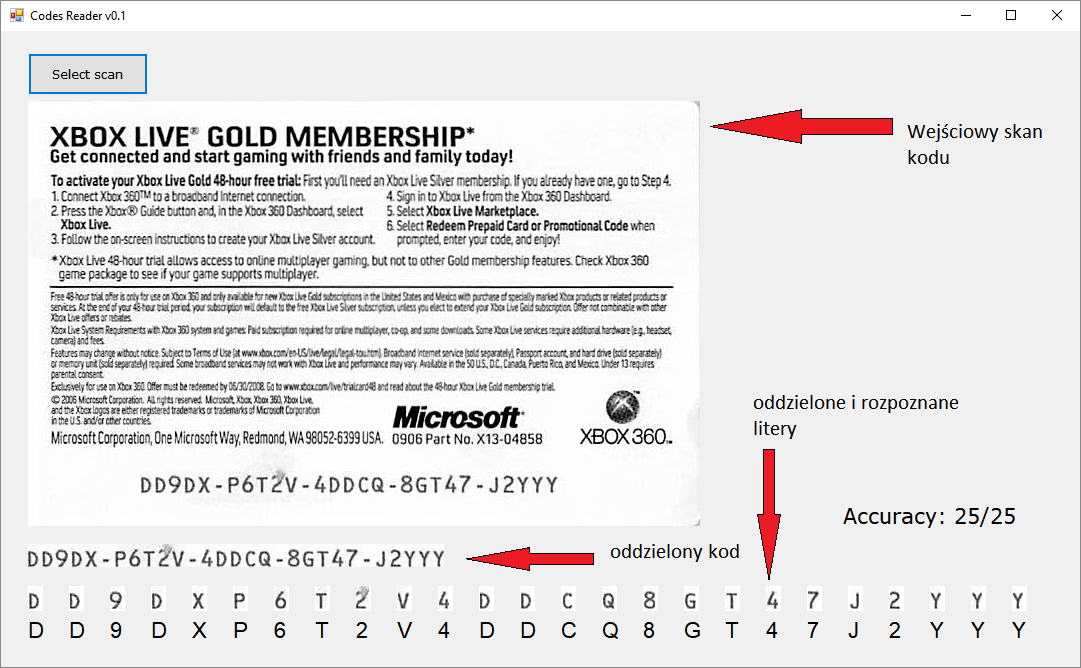
\includegraphics[scale=0.67]{foto1.png}
}


\section{Implementacja}
\subsection{Segmentacja i filtracja skanów}

Segmentacja kodu polegała na przeprowadzeniu następujących operacji na bitmapie:
\begin{enumerate}
	\item Threshold ze stałym progiem (204 i 153)
	\item Usunięcie zanieczyszczeń (obiektów mniejszych niż 8 połączonych pikseli)
	\item Operacja morfologiczna: otwarcie z obiektem strukturalnym o rozmiarze 45x1. Dzięki temu tekst był rozciągnięty tylko w płaszczyźnie poziomej.
	\item Czyszczenie brzegu - dzięki tej operacji usuwaliśmy niepotrzebny tekst ze skanu
	\item Operacja morfologiczna: otwarcie z elementem strukturalnym o rozmiarze 1x5. Dzięki temu uzupełnialiśmy drobne pionowe szczeliny
	\item Wyszukanie największego obiektu na obrazie dawało poszukiwany kod
\end{enumerate}

Segmentacja poszczególnych liter polegała na przeprowadzeniu następujących operacji na bitmapie:
\begin{enumerate}
	\item Adaptive threshold
	\item Usunięcie zanieczyszczeń (obiektów mniejszych niż 8 połączonych pikseli)
	\item Operacja morfologiczna: otwarcie z obiektem strukturalnym o rozmiarze 1x7. Dzięki temu tekst był rozciągnięty tylko w płaszczyźnie pionowej.
	\item Wyodrębnienie obiektów, które dotykały górnej i dolnej krawędzi obrazka dawało nam poszczególne litery
\end{enumerate}

\subsection{SVM i sieć neuronowa}
Do trenowania wykorzystaiśmy 2000 ręcznie przepisanych skanów (łącznie 50 000 liter). Validation set stanowił 20\% zbioru treningowego.
Trenowanie SVM przeprowadziliśmy przy pomocy biblioteki OpenCV. Wykorzystaliśmy tzw grid search aby znaleźć jak najlepsze parametry dla naszego modelu. W wyniku otrzymaliśmy następujące wartości:

Funkcja: wielomian 3 stopnia

Gamma (jak bardzo jeden przykład wpływa na postęp uczenia) : 0.1

Współczynnik0: 1.0

C (jak bardzo każemy SVM za błędne klasyfikacje): 1.0


Trenowanie rekurencyjnej jak i zwykłej sieci neuronowej polegało głównie na eksperymentowaniu w ilości warstw, ilości neuronów w poszczególnych warstwach, sposobu ich łączenia oraz zmian parametrów uczenia (learning rate itd).
Całość wykonaliśmy przy użyciu frameworka TensorFlow. Po wybraniu sieci, która najlepiej się sprawowała na validation set zapisywaliśmy jej model. Następnie porównywaliśmy ją z wcześniej opisanym SVM.


\section {Przykłady wyników}
\subsection{Przykład 1}
Zdjęcia przedstawiają kolejno: SVM, sieć neuronową oraz rekurencyjną sieć neuronową. Najlepiej poradziła sobie sieć neuronowa.
\pagebreak

{\begin{figure}[!htbp]
		\centering
		\caption{Przykład 1 - SVM}
		\vspace{1cm}
		\hspace*{-2.8cm}
		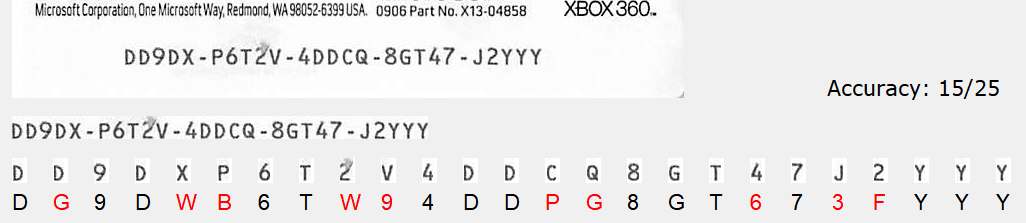
\includegraphics[scale=0.52]{sample1_svm.png}
	\end{figure}
{\begin{figure}[!htbp]
	\centering
		\caption{Przykład 1 - NN}
	\vspace{1cm}
	\hspace*{-2.8cm}
	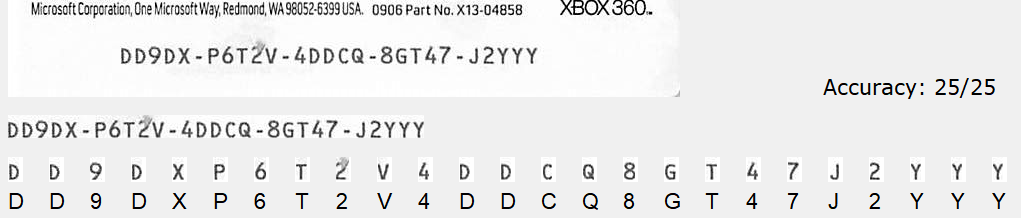
\includegraphics[scale=0.52]{sample1_nn.png}
\end{figure}
}
{\begin{figure}[!htbp]
		\centering
		\caption{Przykład 1 - RNN}
		\vspace{1cm}
		\hspace*{-2.8cm}
		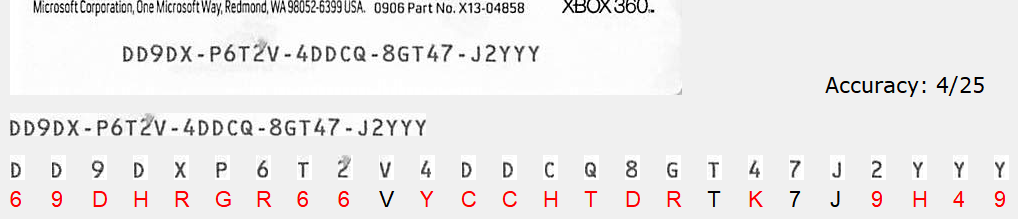
\includegraphics[scale=0.52]{sample1_rnn.png}
	\end{figure}

\pagebreak


\subsection{Przykład 2}
Zdjęcia przedstawiają kolejno: SVM, sieć neuronową oraz rekurencyjną sieć neuronową. Najlepiej poradziła sobie rekurencyjna sieć neuronowa, która mimo zniekształceń była w stanie rozpoznać nawet rozmazane znaki.


{\begin{figure}[!htbp]
		\centering
		\caption{Przykład 2 - SVM}
		\vspace{1cm}
		\hspace*{-2.8cm}
		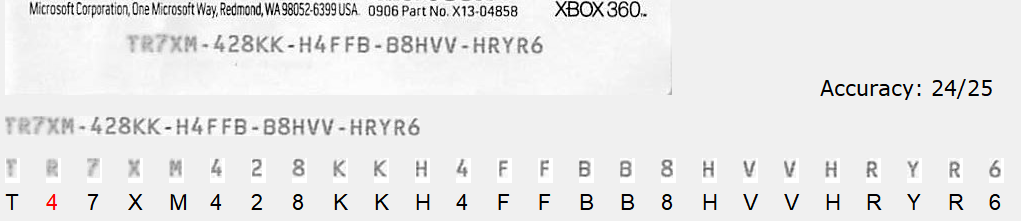
\includegraphics[scale=0.52]{sample2_svm.png}
	\end{figure}
	{\begin{figure}[!htbp]
			\centering
			\caption{Przykład 2 - NN}
			\vspace{1cm}
			\hspace*{-2.8cm}
			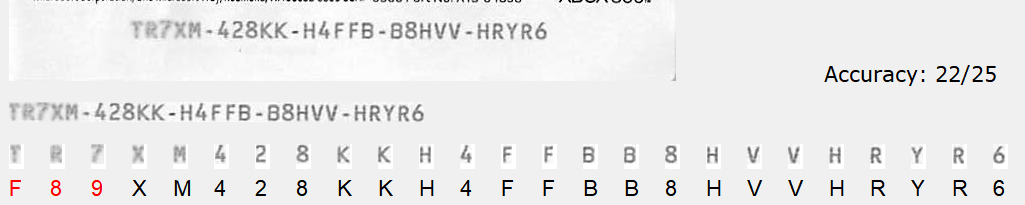
\includegraphics[scale=0.52]{sample2_nn.png}
		\end{figure}
	}
	{\begin{figure}[!htbp]
			\centering
			\caption{Przykład 2 - RNN}
			\vspace{1cm}
			\hspace*{-2.8cm}
			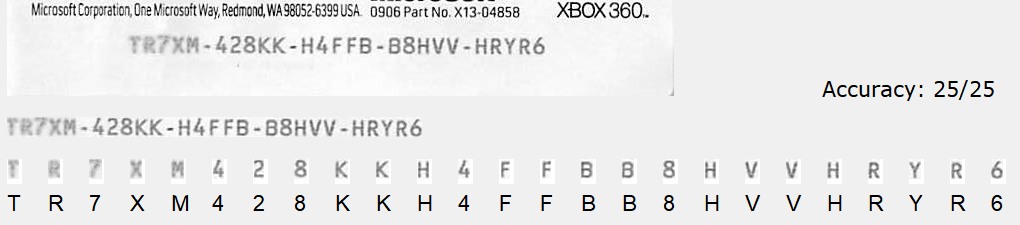
\includegraphics[scale=0.52]{sample2_rnn.png}
		\end{figure}
\pagebreak
\section{Wnioski}
Naszym celem było osiągnięcie jak największej skuteczności w rozpoznaniu kodów z prawie 20 000 skanów (488 225 znaków). Użyliśmy czterech różnych podejść do tego problemu:

\begin{enumerate}
	\item TesseractOCR - jest to silnik OCR, który niestety osiągnął skuteczność zaledwie kilku procent na naszych danych walidacyjnych
	\item Rekurencyjna sieć neuronowa - było to podejście do problemu, które pozwalało pominąć segmentację poszczególnych liter. Niestety przez to złożoność problemu dla sieci znacznie wzrosła i nie poradziła sobie tak dobrze jak zwykła sieć neuronowa czy SVM osiągają skuteczność na poziomie 98,9195\% i myląc się w 211 przypadkach
	\item SVM - osiągnął skuteczność na poziomie 99,7952\% myląc się tylko w 40 przypadkach
	\item Sieć neuronowa - osiągnęła najlepszą skuteczność ze wszystkich metod aż 99,831\% myląc się w 33 przypadkach
\end{enumerate}

Podsumowując projekt można powiedzieć, że sieci neuronowe zdecydowanie sprawdzają się w problemach związanych z rozpoznawaniem tekstu ze zdjęć/skanów. Potrafiły sobie poradzić z dość trudnymi przypadkami liter (często bardzo rozmazanych). Niestety dużym problemem wciąż pozostaje efekt "czarnej skrzynki" przez co ciężko jest efektywnie i szybko zaprojektować sieć, która rozwiąże postawiony przez nas problem.
\end{document}
